\documentclass[11pt,aspectratio=169]{beamer}
% =============================================================================
%  Shared Beamer preamble — Machine Learning I & II, PEU-CD 2026 (ENEI / INEI)
%
%  Inherited from the ML_Foundations deck (Alexander Quispe), with three changes:
%    * `minted` removed — it shells out to Pygments and does not build under
%      tectonic; every code block in the course uses `listings`.
%    * unused packages (lipsum, blindtext, multimedia, videoframe) dropped.
%    * `bbm` dropped — its fonts are PK-only and tectonic cannot render them;
%      the indicator uses \mathbf{1} instead.
%    * a math-macro block added so all twelve lectures share one notation.
%
%  Each lecture is a standalone document:
%      \documentclass[11pt,aspectratio=169]{beamer}
%      % =============================================================================
%  Shared Beamer preamble — Machine Learning I & II, PEU-CD 2026 (ENEI / INEI)
%
%  Inherited from the ML_Foundations deck (Alexander Quispe), with three changes:
%    * `minted` removed — it shells out to Pygments and does not build under
%      tectonic; every code block in the course uses `listings`.
%    * unused packages (lipsum, blindtext, multimedia, videoframe) dropped.
%    * `bbm` dropped — its fonts are PK-only and tectonic cannot render them;
%      the indicator uses \mathbf{1} instead.
%    * a math-macro block added so all twelve lectures share one notation.
%
%  Each lecture is a standalone document:
%      \documentclass[11pt,aspectratio=169]{beamer}
%      % =============================================================================
%  Shared Beamer preamble — Machine Learning I & II, PEU-CD 2026 (ENEI / INEI)
%
%  Inherited from the ML_Foundations deck (Alexander Quispe), with three changes:
%    * `minted` removed — it shells out to Pygments and does not build under
%      tectonic; every code block in the course uses `listings`.
%    * unused packages (lipsum, blindtext, multimedia, videoframe) dropped.
%    * `bbm` dropped — its fonts are PK-only and tectonic cannot render them;
%      the indicator uses \mathbf{1} instead.
%    * a math-macro block added so all twelve lectures share one notation.
%
%  Each lecture is a standalone document:
%      \documentclass[11pt,aspectratio=169]{beamer}
%      \input{../../../style/preamble}
% =============================================================================

% ---------- fonts ----------
\usepackage{helvet}
\usepackage[default]{lato}
\usepackage{tgbonum}
\usepackage{mathpazo}
\usepackage[utf8]{inputenc}

% ---------- math ----------
\usepackage{amsmath,amssymb}
\usepackage{mathtools}

% ---------- graphics, tables, layout ----------
\usepackage{graphicx}
\usepackage{tikz}
\usetikzlibrary{positioning,calc,arrows,arrows.meta,decorations.markings,shapes.misc,matrix,shapes,fit}
\usepackage{array}
\usepackage{booktabs}
\usepackage{multirow}
\usepackage{dcolumn}
\usepackage{subcaption}
\usepackage{caption}
\usepackage{changepage}
\usepackage{xspace}
\usepackage{tcolorbox}
\tcbuselibrary{skins,breakable}
\usepackage[ruled,vlined]{algorithm2e}
\usepackage{listings}
\usepackage{appendixnumberbeamer}
\usepackage{hyperref}

\newcolumntype{d}[0]{D{.}{.}{5}}
\setbeamertemplate{caption}[numbered]

% ---------- palette (Okabe–Ito, colour-blind safe) ----------
\definecolor{blue}{RGB}{0,114,178}
\definecolor{red}{RGB}{213,94,0}
\definecolor{yellow}{RGB}{240,228,66}
\definecolor{green}{RGB}{0,158,115}
\definecolor{MyBackground}{RGB}{255,253,218}

\hypersetup{colorlinks=true, linkbordercolor={white}, linkcolor={blue}, urlcolor={blue}}

% ---------- beamer look ----------
\setbeamercolor{frametitle}{fg=blue}
\setbeamercolor{title}{fg=black}
\setbeamertemplate{footline}[frame number]
\setbeamertemplate{navigation symbols}{}
\setbeamertemplate{itemize items}{-}
\setbeamercolor{itemize item}{fg=blue}
\setbeamercolor{itemize subitem}{fg=blue}
\setbeamercolor{enumerate item}{fg=blue}
\setbeamercolor{enumerate subitem}{fg=blue}
\setbeamercolor{button}{bg=MyBackground,fg=blue}
\setbeamercolor{section in toc}{fg=blue}
\setbeamercolor{subsection in toc}{fg=red}
\setbeamersize{text margin left=1em,text margin right=1em}
\setbeamercolor{block title}{fg=white,bg=blue}
\setbeamercolor{block body}{bg=blue!5}
\setbeamercolor{block title alerted}{fg=white,bg=red}
\setbeamercolor{block body alerted}{bg=red!5}
\setbeamercolor{block title example}{fg=white,bg=green}
\setbeamercolor{block body example}{bg=green!5}
\setbeamertemplate{blocks}[rounded][shadow=false]

\newenvironment{wideitemize}{\itemize\addtolength{\itemsep}{10pt}}{\enditemize}

\newenvironment{transitionframe}{
  \setbeamercolor{background canvas}{bg=yellow}
  \begin{frame}}{
  \end{frame}
}

% Section divider: a plain frame with a large blue title.
\newcommand{\sectionframe}[1]{%
  \section{#1}%
  \begin{frame}[plain]\vfill\begin{center}{\Huge\textcolor{blue}{#1}}\end{center}\vfill\end{frame}}

% ---------- proof / derivation environments ----------
% derivation: a boxed, step-by-step algebraic argument. Title is the claim.
\newtcolorbox{derivation}[1]{enhanced, colback=blue!3, colframe=blue, fonttitle=\bfseries,
  title={#1}, boxrule=0.6pt, left=4pt, right=4pt, top=3pt, bottom=3pt, arc=2pt}
% claim: a result to be proved (theorem / lemma / proposition).
\newtcolorbox{claim}[1]{enhanced, colback=white, colframe=black, fonttitle=\bfseries,
  title={#1}, boxrule=0.6pt, left=4pt, right=4pt, top=3pt, bottom=3pt, arc=2pt}
% keypoint: the one line to remember from a slide.
\newtcolorbox{keypoint}{enhanced, colback=green!6, colframe=green, boxrule=0.6pt,
  left=4pt, right=4pt, top=3pt, bottom=3pt, arc=2pt}
% caution: a common mistake or a subtlety.
\newtcolorbox{caution}{enhanced, colback=red!5, colframe=red, boxrule=0.6pt,
  left=4pt, right=4pt, top=3pt, bottom=3pt, arc=2pt}

% ---------- code ----------
\lstset{
  basicstyle=\ttfamily\scriptsize, keywordstyle=\color{blue}\bfseries,
  commentstyle=\color{green}, stringstyle=\color{red},
  showstringspaces=false, breaklines=true, frame=single, rulecolor=\color{black!30},
  numbers=none, xleftmargin=4pt, framexleftmargin=4pt, language=Python
}

\input{../../../style/macros}

% ---------- course-wide title metadata ----------
\newcommand{\courseinstitution}{ENEI -- INEI \,\textperiodcentered\, PEU-CD 2026}
\newcommand{\courseauthor}{Alexander Quispe}
\institute{\courseinstitution}
\author{\courseauthor}

% =============================================================================

% ---------- fonts ----------
\usepackage{helvet}
\usepackage[default]{lato}
\usepackage{tgbonum}
\usepackage{mathpazo}
\usepackage[utf8]{inputenc}

% ---------- math ----------
\usepackage{amsmath,amssymb}
\usepackage{mathtools}

% ---------- graphics, tables, layout ----------
\usepackage{graphicx}
\usepackage{tikz}
\usetikzlibrary{positioning,calc,arrows,arrows.meta,decorations.markings,shapes.misc,matrix,shapes,fit}
\usepackage{array}
\usepackage{booktabs}
\usepackage{multirow}
\usepackage{dcolumn}
\usepackage{subcaption}
\usepackage{caption}
\usepackage{changepage}
\usepackage{xspace}
\usepackage{tcolorbox}
\tcbuselibrary{skins,breakable}
\usepackage[ruled,vlined]{algorithm2e}
\usepackage{listings}
\usepackage{appendixnumberbeamer}
\usepackage{hyperref}

\newcolumntype{d}[0]{D{.}{.}{5}}
\setbeamertemplate{caption}[numbered]

% ---------- palette (Okabe–Ito, colour-blind safe) ----------
\definecolor{blue}{RGB}{0,114,178}
\definecolor{red}{RGB}{213,94,0}
\definecolor{yellow}{RGB}{240,228,66}
\definecolor{green}{RGB}{0,158,115}
\definecolor{MyBackground}{RGB}{255,253,218}

\hypersetup{colorlinks=true, linkbordercolor={white}, linkcolor={blue}, urlcolor={blue}}

% ---------- beamer look ----------
\setbeamercolor{frametitle}{fg=blue}
\setbeamercolor{title}{fg=black}
\setbeamertemplate{footline}[frame number]
\setbeamertemplate{navigation symbols}{}
\setbeamertemplate{itemize items}{-}
\setbeamercolor{itemize item}{fg=blue}
\setbeamercolor{itemize subitem}{fg=blue}
\setbeamercolor{enumerate item}{fg=blue}
\setbeamercolor{enumerate subitem}{fg=blue}
\setbeamercolor{button}{bg=MyBackground,fg=blue}
\setbeamercolor{section in toc}{fg=blue}
\setbeamercolor{subsection in toc}{fg=red}
\setbeamersize{text margin left=1em,text margin right=1em}
\setbeamercolor{block title}{fg=white,bg=blue}
\setbeamercolor{block body}{bg=blue!5}
\setbeamercolor{block title alerted}{fg=white,bg=red}
\setbeamercolor{block body alerted}{bg=red!5}
\setbeamercolor{block title example}{fg=white,bg=green}
\setbeamercolor{block body example}{bg=green!5}
\setbeamertemplate{blocks}[rounded][shadow=false]

\newenvironment{wideitemize}{\itemize\addtolength{\itemsep}{10pt}}{\enditemize}

\newenvironment{transitionframe}{
  \setbeamercolor{background canvas}{bg=yellow}
  \begin{frame}}{
  \end{frame}
}

% Section divider: a plain frame with a large blue title.
\newcommand{\sectionframe}[1]{%
  \section{#1}%
  \begin{frame}[plain]\vfill\begin{center}{\Huge\textcolor{blue}{#1}}\end{center}\vfill\end{frame}}

% ---------- proof / derivation environments ----------
% derivation: a boxed, step-by-step algebraic argument. Title is the claim.
\newtcolorbox{derivation}[1]{enhanced, colback=blue!3, colframe=blue, fonttitle=\bfseries,
  title={#1}, boxrule=0.6pt, left=4pt, right=4pt, top=3pt, bottom=3pt, arc=2pt}
% claim: a result to be proved (theorem / lemma / proposition).
\newtcolorbox{claim}[1]{enhanced, colback=white, colframe=black, fonttitle=\bfseries,
  title={#1}, boxrule=0.6pt, left=4pt, right=4pt, top=3pt, bottom=3pt, arc=2pt}
% keypoint: the one line to remember from a slide.
\newtcolorbox{keypoint}{enhanced, colback=green!6, colframe=green, boxrule=0.6pt,
  left=4pt, right=4pt, top=3pt, bottom=3pt, arc=2pt}
% caution: a common mistake or a subtlety.
\newtcolorbox{caution}{enhanced, colback=red!5, colframe=red, boxrule=0.6pt,
  left=4pt, right=4pt, top=3pt, bottom=3pt, arc=2pt}

% ---------- code ----------
\lstset{
  basicstyle=\ttfamily\scriptsize, keywordstyle=\color{blue}\bfseries,
  commentstyle=\color{green}, stringstyle=\color{red},
  showstringspaces=false, breaklines=true, frame=single, rulecolor=\color{black!30},
  numbers=none, xleftmargin=4pt, framexleftmargin=4pt, language=Python
}

% =============================================================================
%  Notation — one convention for all lectures
%
%  scalars      x, y, w           plain italic
%  vectors      \vx \vy \vw       bold lower-case
%  matrices     \vX \vW \vSigma   bold upper-case
%  parameters   \vbeta \vtheta    bold Greek
%  transpose    \vX\T             \top
% =============================================================================
\newcommand{\R}{\mathbb{R}}
\newcommand{\E}{\mathbb{E}}
\newcommand{\Prob}{\mathbb{P}}
\DeclareMathOperator{\Var}{Var}
\DeclareMathOperator{\Cov}{Cov}
\DeclareMathOperator{\tr}{tr}
\DeclareMathOperator{\diag}{diag}
\DeclareMathOperator{\rank}{rank}
\DeclareMathOperator{\sign}{sign}
\DeclareMathOperator{\col}{col}
\DeclareMathOperator{\RSS}{RSS}
\DeclareMathOperator*{\argmin}{arg\,min}
\DeclareMathOperator*{\argmax}{arg\,max}
\newcommand{\norm}[1]{\left\lVert #1 \right\rVert}
\newcommand{\abs}[1]{\left\lvert #1 \right\rvert}
\newcommand{\inner}[2]{\left\langle #1,\, #2 \right\rangle}
\newcommand{\ind}[1]{\mathbf{1}\!\left\{#1\right\}}
\newcommand{\T}{^{\top}}
\newcommand{\inv}{^{-1}}
\newcommand{\half}{\tfrac{1}{2}}
\newcommand{\eps}{\varepsilon}
\newcommand{\Dset}{\mathcal{D}}
\newcommand{\Hset}{\mathcal{H}}
\newcommand{\Lcal}{\mathcal{L}}
\newcommand{\Ncal}{\mathcal{N}}

% bold vectors
\newcommand{\vx}{\mathbf{x}}   \newcommand{\vy}{\mathbf{y}}   \newcommand{\vz}{\mathbf{z}}
\newcommand{\vw}{\mathbf{w}}   \newcommand{\vu}{\mathbf{u}}   \newcommand{\vv}{\mathbf{v}}
\newcommand{\vb}{\mathbf{b}}   \newcommand{\vh}{\mathbf{h}}   \newcommand{\vr}{\mathbf{r}}
\newcommand{\vc}{\mathbf{c}}   \newcommand{\vf}{\mathbf{f}}   \newcommand{\vg}{\mathbf{g}}
\newcommand{\vp}{\mathbf{p}}   \newcommand{\vq}{\mathbf{q}}   \newcommand{\vs}{\mathbf{s}}
\newcommand{\va}{\mathbf{a}}   \newcommand{\vd}{\mathbf{d}}   \newcommand{\vt}{\mathbf{t}}
\newcommand{\vk}{\mathbf{k}}   \newcommand{\vm}{\mathbf{m}}   \newcommand{\vn}{\mathbf{n}}
\newcommand{\vzero}{\mathbf{0}} \newcommand{\vone}{\mathbf{1}}
% bold matrices
\newcommand{\vX}{\mathbf{X}}   \newcommand{\vY}{\mathbf{Y}}   \newcommand{\vZ}{\mathbf{Z}}
\newcommand{\vW}{\mathbf{W}}   \newcommand{\vH}{\mathbf{H}}   \newcommand{\vI}{\mathbf{I}}
\newcommand{\vA}{\mathbf{A}}   \newcommand{\vB}{\mathbf{B}}   \newcommand{\vC}{\mathbf{C}}
\newcommand{\vD}{\mathbf{D}}   \newcommand{\vP}{\mathbf{P}}   \newcommand{\vQ}{\mathbf{Q}}
\newcommand{\vU}{\mathbf{U}}   \newcommand{\vV}{\mathbf{V}}   \newcommand{\vS}{\mathbf{S}}
\newcommand{\vM}{\mathbf{M}}   \newcommand{\vK}{\mathbf{K}}   \newcommand{\vG}{\mathbf{G}}
% bold Greek
\newcommand{\vbeta}{\boldsymbol{\beta}}     \newcommand{\valpha}{\boldsymbol{\alpha}}
\newcommand{\vtheta}{\boldsymbol{\theta}}   \newcommand{\vmu}{\boldsymbol{\mu}}
\newcommand{\vSigma}{\boldsymbol{\Sigma}}   \newcommand{\vLambda}{\boldsymbol{\Lambda}}
\newcommand{\veps}{\boldsymbol{\varepsilon}} \newcommand{\vphi}{\boldsymbol{\phi}}
\newcommand{\vgamma}{\boldsymbol{\gamma}}   \newcommand{\vlambda}{\boldsymbol{\lambda}}
\newcommand{\vdelta}{\boldsymbol{\delta}}   \newcommand{\vnu}{\boldsymbol{\nu}}
\newcommand{\vxi}{\boldsymbol{\xi}}         \newcommand{\vpi}{\boldsymbol{\pi}}
\newcommand{\vomega}{\boldsymbol{\omega}}



% ---------- course-wide title metadata ----------
\newcommand{\courseinstitution}{ENEI -- INEI \,\textperiodcentered\, PEU-CD 2026}
\newcommand{\courseauthor}{Alexander Quispe}
\institute{\courseinstitution}
\author{\courseauthor}

% =============================================================================

% ---------- fonts ----------
\usepackage{helvet}
\usepackage[default]{lato}
\usepackage{tgbonum}
\usepackage{mathpazo}
\usepackage[utf8]{inputenc}

% ---------- math ----------
\usepackage{amsmath,amssymb}
\usepackage{mathtools}

% ---------- graphics, tables, layout ----------
\usepackage{graphicx}
\usepackage{tikz}
\usetikzlibrary{positioning,calc,arrows,arrows.meta,decorations.markings,shapes.misc,matrix,shapes,fit}
\usepackage{array}
\usepackage{booktabs}
\usepackage{multirow}
\usepackage{dcolumn}
\usepackage{subcaption}
\usepackage{caption}
\usepackage{changepage}
\usepackage{xspace}
\usepackage{tcolorbox}
\tcbuselibrary{skins,breakable}
\usepackage[ruled,vlined]{algorithm2e}
\usepackage{listings}
\usepackage{appendixnumberbeamer}
\usepackage{hyperref}

\newcolumntype{d}[0]{D{.}{.}{5}}
\setbeamertemplate{caption}[numbered]

% ---------- palette (Okabe–Ito, colour-blind safe) ----------
\definecolor{blue}{RGB}{0,114,178}
\definecolor{red}{RGB}{213,94,0}
\definecolor{yellow}{RGB}{240,228,66}
\definecolor{green}{RGB}{0,158,115}
\definecolor{MyBackground}{RGB}{255,253,218}

\hypersetup{colorlinks=true, linkbordercolor={white}, linkcolor={blue}, urlcolor={blue}}

% ---------- beamer look ----------
\setbeamercolor{frametitle}{fg=blue}
\setbeamercolor{title}{fg=black}
\setbeamertemplate{footline}[frame number]
\setbeamertemplate{navigation symbols}{}
\setbeamertemplate{itemize items}{-}
\setbeamercolor{itemize item}{fg=blue}
\setbeamercolor{itemize subitem}{fg=blue}
\setbeamercolor{enumerate item}{fg=blue}
\setbeamercolor{enumerate subitem}{fg=blue}
\setbeamercolor{button}{bg=MyBackground,fg=blue}
\setbeamercolor{section in toc}{fg=blue}
\setbeamercolor{subsection in toc}{fg=red}
\setbeamersize{text margin left=1em,text margin right=1em}
\setbeamercolor{block title}{fg=white,bg=blue}
\setbeamercolor{block body}{bg=blue!5}
\setbeamercolor{block title alerted}{fg=white,bg=red}
\setbeamercolor{block body alerted}{bg=red!5}
\setbeamercolor{block title example}{fg=white,bg=green}
\setbeamercolor{block body example}{bg=green!5}
\setbeamertemplate{blocks}[rounded][shadow=false]

\newenvironment{wideitemize}{\itemize\addtolength{\itemsep}{10pt}}{\enditemize}

\newenvironment{transitionframe}{
  \setbeamercolor{background canvas}{bg=yellow}
  \begin{frame}}{
  \end{frame}
}

% Section divider: a plain frame with a large blue title.
\newcommand{\sectionframe}[1]{%
  \section{#1}%
  \begin{frame}[plain]\vfill\begin{center}{\Huge\textcolor{blue}{#1}}\end{center}\vfill\end{frame}}

% ---------- proof / derivation environments ----------
% derivation: a boxed, step-by-step algebraic argument. Title is the claim.
\newtcolorbox{derivation}[1]{enhanced, colback=blue!3, colframe=blue, fonttitle=\bfseries,
  title={#1}, boxrule=0.6pt, left=4pt, right=4pt, top=3pt, bottom=3pt, arc=2pt}
% claim: a result to be proved (theorem / lemma / proposition).
\newtcolorbox{claim}[1]{enhanced, colback=white, colframe=black, fonttitle=\bfseries,
  title={#1}, boxrule=0.6pt, left=4pt, right=4pt, top=3pt, bottom=3pt, arc=2pt}
% keypoint: the one line to remember from a slide.
\newtcolorbox{keypoint}{enhanced, colback=green!6, colframe=green, boxrule=0.6pt,
  left=4pt, right=4pt, top=3pt, bottom=3pt, arc=2pt}
% caution: a common mistake or a subtlety.
\newtcolorbox{caution}{enhanced, colback=red!5, colframe=red, boxrule=0.6pt,
  left=4pt, right=4pt, top=3pt, bottom=3pt, arc=2pt}

% ---------- code ----------
\lstset{
  basicstyle=\ttfamily\scriptsize, keywordstyle=\color{blue}\bfseries,
  commentstyle=\color{green}, stringstyle=\color{red},
  showstringspaces=false, breaklines=true, frame=single, rulecolor=\color{black!30},
  numbers=none, xleftmargin=4pt, framexleftmargin=4pt, language=Python
}

% =============================================================================
%  Notation — one convention for all lectures
%
%  scalars      x, y, w           plain italic
%  vectors      \vx \vy \vw       bold lower-case
%  matrices     \vX \vW \vSigma   bold upper-case
%  parameters   \vbeta \vtheta    bold Greek
%  transpose    \vX\T             \top
% =============================================================================
\newcommand{\R}{\mathbb{R}}
\newcommand{\E}{\mathbb{E}}
\newcommand{\Prob}{\mathbb{P}}
\DeclareMathOperator{\Var}{Var}
\DeclareMathOperator{\Cov}{Cov}
\DeclareMathOperator{\tr}{tr}
\DeclareMathOperator{\diag}{diag}
\DeclareMathOperator{\rank}{rank}
\DeclareMathOperator{\sign}{sign}
\DeclareMathOperator{\col}{col}
\DeclareMathOperator{\RSS}{RSS}
\DeclareMathOperator*{\argmin}{arg\,min}
\DeclareMathOperator*{\argmax}{arg\,max}
\newcommand{\norm}[1]{\left\lVert #1 \right\rVert}
\newcommand{\abs}[1]{\left\lvert #1 \right\rvert}
\newcommand{\inner}[2]{\left\langle #1,\, #2 \right\rangle}
\newcommand{\ind}[1]{\mathbf{1}\!\left\{#1\right\}}
\newcommand{\T}{^{\top}}
\newcommand{\inv}{^{-1}}
\newcommand{\half}{\tfrac{1}{2}}
\newcommand{\eps}{\varepsilon}
\newcommand{\Dset}{\mathcal{D}}
\newcommand{\Hset}{\mathcal{H}}
\newcommand{\Lcal}{\mathcal{L}}
\newcommand{\Ncal}{\mathcal{N}}

% bold vectors
\newcommand{\vx}{\mathbf{x}}   \newcommand{\vy}{\mathbf{y}}   \newcommand{\vz}{\mathbf{z}}
\newcommand{\vw}{\mathbf{w}}   \newcommand{\vu}{\mathbf{u}}   \newcommand{\vv}{\mathbf{v}}
\newcommand{\vb}{\mathbf{b}}   \newcommand{\vh}{\mathbf{h}}   \newcommand{\vr}{\mathbf{r}}
\newcommand{\vc}{\mathbf{c}}   \newcommand{\vf}{\mathbf{f}}   \newcommand{\vg}{\mathbf{g}}
\newcommand{\vp}{\mathbf{p}}   \newcommand{\vq}{\mathbf{q}}   \newcommand{\vs}{\mathbf{s}}
\newcommand{\va}{\mathbf{a}}   \newcommand{\vd}{\mathbf{d}}   \newcommand{\vt}{\mathbf{t}}
\newcommand{\vk}{\mathbf{k}}   \newcommand{\vm}{\mathbf{m}}   \newcommand{\vn}{\mathbf{n}}
\newcommand{\vzero}{\mathbf{0}} \newcommand{\vone}{\mathbf{1}}
% bold matrices
\newcommand{\vX}{\mathbf{X}}   \newcommand{\vY}{\mathbf{Y}}   \newcommand{\vZ}{\mathbf{Z}}
\newcommand{\vW}{\mathbf{W}}   \newcommand{\vH}{\mathbf{H}}   \newcommand{\vI}{\mathbf{I}}
\newcommand{\vA}{\mathbf{A}}   \newcommand{\vB}{\mathbf{B}}   \newcommand{\vC}{\mathbf{C}}
\newcommand{\vD}{\mathbf{D}}   \newcommand{\vP}{\mathbf{P}}   \newcommand{\vQ}{\mathbf{Q}}
\newcommand{\vU}{\mathbf{U}}   \newcommand{\vV}{\mathbf{V}}   \newcommand{\vS}{\mathbf{S}}
\newcommand{\vM}{\mathbf{M}}   \newcommand{\vK}{\mathbf{K}}   \newcommand{\vG}{\mathbf{G}}
% bold Greek
\newcommand{\vbeta}{\boldsymbol{\beta}}     \newcommand{\valpha}{\boldsymbol{\alpha}}
\newcommand{\vtheta}{\boldsymbol{\theta}}   \newcommand{\vmu}{\boldsymbol{\mu}}
\newcommand{\vSigma}{\boldsymbol{\Sigma}}   \newcommand{\vLambda}{\boldsymbol{\Lambda}}
\newcommand{\veps}{\boldsymbol{\varepsilon}} \newcommand{\vphi}{\boldsymbol{\phi}}
\newcommand{\vgamma}{\boldsymbol{\gamma}}   \newcommand{\vlambda}{\boldsymbol{\lambda}}
\newcommand{\vdelta}{\boldsymbol{\delta}}   \newcommand{\vnu}{\boldsymbol{\nu}}
\newcommand{\vxi}{\boldsymbol{\xi}}         \newcommand{\vpi}{\boldsymbol{\pi}}
\newcommand{\vomega}{\boldsymbol{\omega}}



% ---------- course-wide title metadata ----------
\newcommand{\courseinstitution}{ENEI -- INEI \,\textperiodcentered\, PEU-CD 2026}
\newcommand{\courseauthor}{Alexander Quispe}
\institute{\courseinstitution}
\author{\courseauthor}

\graphicspath{{figures/}}

\title{\textcolor{blue}{Lecture 5 \\ Boosting}}
\subtitle{Machine Learning I}
\date{September 21, 2026}

\begin{document}

\begin{frame}[plain]
\maketitle
\end{frame}

\begin{frame}{Outline}
\tableofcontents
\end{frame}

\begin{frame}{Two Ways to Combine Models}
\begin{columns}[T]
\begin{column}{0.48\textwidth}
\textbf{Bagging (Lecture 4)}
\begin{itemize}
  \item Many \emph{independent} deep trees.
  \item Each: low bias, high variance.
  \item Average them. Variance $\to\rho\sigma^2$, bias unchanged.
  \item Parallel; order does not matter.
\end{itemize}
\end{column}
\begin{column}{0.48\textwidth}
\textbf{Boosting (today)}
\begin{itemize}
  \item Many \emph{dependent} shallow trees.
  \item Each: high bias, low variance.
  \item Add them one at a time, each correcting the last. Bias falls; variance is controlled by the step size.
  \item Sequential; order is everything.
\end{itemize}
\end{column}
\end{columns}
\vspace{10pt}
\begin{block}{The question (Kearns \& Valiant, 1988)}
If a learner can always do slightly better than chance, can it be turned into one that does arbitrarily well?
\end{block}
Schapire (1990) proved yes. AdaBoost (Freund \& Schapire, 1995) made it practical. Gradient boosting
(Friedman, 2001) explained what it was doing. We take them in reverse order.
\end{frame}

% =============================================================================
\sectionframe{Additive Models and Forward Stagewise Fitting}
% =============================================================================

\begin{frame}{Additive Models}
The hypothesis class is sums of $M$ \textbf{base learners} from a simple class $\Hset_0$
(stumps, depth-3 trees, \dots):
\[
f_M(\vx)=\sum_{m=1}^M\alpha_mh_m(\vx),\qquad h_m\in\Hset_0,\ \alpha_m\in\R .
\]
Fitting all $(\alpha_m,h_m)$ jointly is intractable for trees. Instead, \textbf{forward stagewise}:
\begin{block}{}
\[
(\alpha_m,h_m)=\argmin_{\alpha,h\in\Hset_0}\ \sum_{i=1}^NL\bigl(y_i,\ f_{m-1}(\vx_i)+\alpha h(\vx_i)\bigr),
\qquad f_m=f_{m-1}+\alpha_mh_m .
\]
\end{block}
Freeze what you have; add the one term that helps most. Never revisit.
\end{frame}

\begin{frame}{Squared Loss: Fit the Residuals}\small
\begin{derivation}{Stagewise least squares}
With $L(y,f)=\tfrac12(y-f)^2$ and $r_i^{(m)}=y_i-f_{m-1}(\vx_i)$ the current residuals,
\[
\sum_iL\bigl(y_i,f_{m-1}(\vx_i)+\alpha h(\vx_i)\bigr)=\frac12\sum_i\bigl(r_i^{(m)}-\alpha h(\vx_i)\bigr)^2 .
\]
For $\alpha=1$ this is the least-squares fit of $h$ to the residuals. So: \emph{fit a base learner to
whatever the current model gets wrong, add it, repeat}.
\end{derivation}
\begin{center}
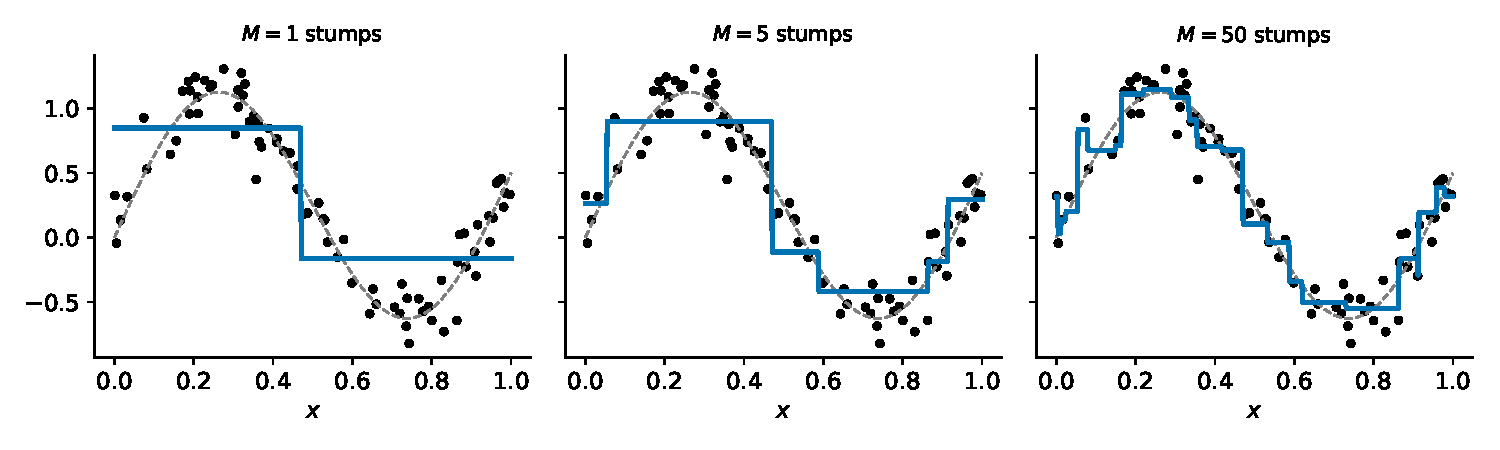
\includegraphics[height=0.3\textheight]{fig_stagewise.pdf}
\end{center}
\vspace{-4pt}
Stumps on a 1-D target. Each stage fits the residual of the previous stage; the sum approaches the curve.
\end{frame}

% =============================================================================
\sectionframe{Gradient Boosting}
% =============================================================================

\begin{frame}{Optimization in Function Space}
Consider the empirical risk as a function of the $N$ fitted values $\vf=(f(\vx_1),\dots,f(\vx_N))\T\in\R^N$:
\[
J(\vf)=\sum_{i=1}^NL(y_i,f_i).
\]
Gradient descent in $\R^N$ would set $\vf\leftarrow\vf-\eta\,\vg$ with
\[
g_i=\frac{\partial L(y_i,f_i)}{\partial f_i}\Big|_{f_i=f_{m-1}(\vx_i)}.
\]
\begin{itemize}
  \item We cannot move $\vf$ freely: the update must be a function $h\in\Hset_0$ evaluated at the $\vx_i$.
  \item So project the step onto $\Hset_0$: choose $h_m$ as the base learner \textbf{closest to $-\vg$},
        in the least-squares sense, then pick the step length by line search.
\end{itemize}
\begin{keypoint}
Boosting is gradient descent in the space of functions, constrained to move along directions the base
learner can represent. The residuals of the previous slide are the special case $-\vg=\vr$ for squared loss.
\end{keypoint}
\end{frame}

\begin{frame}{Gradient Boosting (Friedman, 2001)}\footnotesize
\begin{algorithm}[H]
\SetAlgoLined
\KwIn{data, loss $L$, base class $\Hset_0$, rounds $M$, shrinkage $\nu\in(0,1]$}
$f_0\gets\argmin_c\sum_iL(y_i,c)$ \tcp*{a constant: the mean, the median, the log-odds}
\For{$m=1,\dots,M$}{
  $\tilde r_i\gets-\dfrac{\partial L(y_i,f)}{\partial f}\Big|_{f=f_{m-1}(\vx_i)}$, \ $i=1,\dots,N$ \tcp*{pseudo-residuals}
  $h_m\gets\argmin_{h\in\Hset_0}\sum_i\bigl(\tilde r_i-h(\vx_i)\bigr)^2$ \tcp*{fit a tree to them}
  $\alpha_m\gets\argmin_\alpha\sum_iL\bigl(y_i,f_{m-1}(\vx_i)+\alpha h_m(\vx_i)\bigr)$ \tcp*{line search}
  $f_m\gets f_{m-1}+\nu\,\alpha_mh_m$\;
}
\KwOut{$f_M$}
\end{algorithm}
\begin{center}
\begin{tabular}{lll}
\toprule
Loss & $L(y,f)$ & Pseudo-residual $\tilde r_i=-\partial L/\partial f$ \\
\midrule
Squared & $\tfrac12(y-f)^2$ & $y_i-f(\vx_i)$ \\
Absolute & $\abs{y-f}$ & $\sign\bigl(y_i-f(\vx_i)\bigr)$ \\
Log (binary, $y\in\{0,1\}$) & $-y f+\log(1+e^f)$ & $y_i-\sigma\bigl(f(\vx_i)\bigr)$ \\
Exponential ($y\in\{\pm1\}$) & $e^{-yf}$ & $y_ie^{-y_if(\vx_i)}$ \\
\bottomrule
\end{tabular}
\end{center}
\end{frame}

\begin{frame}{The Knobs}
\begin{description}
  \item[Number of rounds $M$] The main capacity control. Training loss decreases monotonically; validation
        loss eventually rises. Choose $M$ by early stopping on a validation set.
  \item[Shrinkage $\nu$] Scales every step. Small $\nu$ (0.01--0.1) with large $M$ beats $\nu=1$ with small $M$
        at the same training loss --- it behaves like $\ell_2$ regularization on the path (Lecture 3's early-stopping remark).
  \item[Tree depth $d$] Sets the \textbf{interaction order}: a depth-$d$ tree can represent interactions among
        at most $d$ features. Stumps ($d=1$) give an additive model in the features. $d\in[3,8]$ is typical.
  \item[Subsampling] Fit each tree on a random fraction ($\approx0.5$) of the rows: lowers variance and cost
        (\emph{stochastic} gradient boosting). Column subsampling at each split does the same, as in random forests.
\end{description}
\begin{caution}
Unlike random forests, boosting \textbf{does} overfit in $M$. It is the one hyperparameter that must be tuned
every time.
\end{caution}
\end{frame}

\begin{frame}{Second-Order Boosting (XGBoost, 2016)}\footnotesize
Replace the gradient step by a Newton step. At round $m$, expand the loss to second order in the update $h$:
\[
\sum_iL\bigl(y_i,f_{m-1}(\vx_i)+h(\vx_i)\bigr)\approx\sum_i\Bigl[L\bigl(y_i,f_{m-1}(\vx_i)\bigr)+g_ih(\vx_i)+\tfrac12\,k_i\,h(\vx_i)^2\Bigr],
\qquad g_i=\frac{\partial L}{\partial f},\ k_i=\frac{\partial^2L}{\partial f^2}.
\]
\begin{derivation}{Optimal leaf values for a tree with leaves $R_1,\dots,R_T$ and weights $w_1,\dots,w_T$}
$h(\vx)=w_j$ on $R_j$. Add a penalty $\frac\lambda2\sum_jw_j^2+\gamma T$. Writing $G_j=\sum_{i\in R_j}g_i$, $K_j=\sum_{i\in R_j}k_i$:
\[
\sum_{j=1}^T\Bigl[G_jw_j+\tfrac12(K_j+\lambda)w_j^2\Bigr]+\gamma T
\quad\Longrightarrow\quad
\frac{\partial}{\partial w_j}=G_j+(K_j+\lambda)w_j=0
\quad\Longrightarrow\quad
\boxed{w_j^\star=-\frac{G_j}{K_j+\lambda}}
\]
Substituting back, the objective at the optimum is $-\tfrac12\sum_j\dfrac{G_j^2}{K_j+\lambda}+\gamma T$.
\end{derivation}
\begin{keypoint}
The \textbf{gain} of a split $R\to R_L\cup R_R$ is therefore
$\ \tfrac12\Bigl[\tfrac{G_L^2}{K_L+\lambda}+\tfrac{G_R^2}{K_R+\lambda}-\tfrac{G^2}{K+\lambda}\Bigr]-\gamma$:
an impurity function tailored to the loss, derived rather than chosen. Splits with gain $<0$ are pruned.
\end{keypoint}
\end{frame}

% =============================================================================
\sectionframe{AdaBoost}
% =============================================================================

\begin{frame}{The Setting}
Binary labels $y\in\{-1,+1\}$; base learners $h:\R^p\to\{-1,+1\}$ (stumps, typically). Final classifier
\[
H(\vx)=\sign\bigl(f_M(\vx)\bigr),\qquad f_M(\vx)=\sum_{m=1}^M\alpha_mh_m(\vx).
\]
\begin{block}{Weak learner}
Given any distribution $\vw$ over the training points, the base learner returns $h$ with weighted error
\[
\varepsilon=\sum_{i:\,h(\vx_i)\ne y_i}w_i\ \le\ \tfrac12-\gamma,\qquad\gamma>0 .
\]
\end{block}
Slightly better than a coin flip, on \emph{every} reweighting of the data. That is all AdaBoost assumes.
\vspace{6pt}

AdaBoost is forward stagewise fitting with the \textbf{exponential loss} $L(y,f)=e^{-yf}$. Everything below
is derived from that one fact.
\end{frame}

\begin{frame}{Deriving AdaBoost, Part 1: What the Weights Are}\footnotesize
At round $m$, with $f_{m-1}$ fixed, the stagewise objective is
\[
\sum_{i=1}^N\exp\bigl(-y_i[f_{m-1}(\vx_i)+\alpha h(\vx_i)]\bigr)
=\sum_{i=1}^N\underbrace{e^{-y_if_{m-1}(\vx_i)}}_{w_i^{(m)}}\,e^{-\alpha y_ih(\vx_i)} .
\]
\begin{derivation}{Split the sum by whether $h$ is right or wrong}
Since $y_ih(\vx_i)\in\{+1,-1\}$,
\begin{align*}
\sum_iw_i^{(m)}e^{-\alpha y_ih(\vx_i)}
&=e^{-\alpha}\sum_{i:\,h(\vx_i)=y_i}w_i^{(m)}+e^{\alpha}\sum_{i:\,h(\vx_i)\ne y_i}w_i^{(m)}\\
&=e^{-\alpha}\sum_iw_i^{(m)}+\bigl(e^{\alpha}-e^{-\alpha}\bigr)\sum_{i:\,h(\vx_i)\ne y_i}w_i^{(m)} .
\end{align*}
\end{derivation}
For any $\alpha>0$ the first term does not depend on $h$ and the bracket is positive. So the best $h$ is the
one with the smallest \textbf{weighted error} $\varepsilon_m=\sum_{i:\,h(\vx_i)\ne y_i}w_i^{(m)}\big/\sum_iw_i^{(m)}$.
\begin{keypoint}
The weights are the exponential losses of the current model. Points the current model gets badly wrong get
heavy weight; the base learner is told to focus on them.
\end{keypoint}
\end{frame}

\begin{frame}{Deriving AdaBoost, Part 2: What $\alpha$ Is}
Normalize the weights to sum to 1. With $h_m$ chosen, the objective in $\alpha$ is
\[
\phi(\alpha)=(1-\varepsilon_m)e^{-\alpha}+\varepsilon_me^{\alpha}.
\]
\begin{derivation}{Minimize over $\alpha$}
\[
\phi'(\alpha)=-(1-\varepsilon_m)e^{-\alpha}+\varepsilon_me^{\alpha}=0
\quad\Longrightarrow\quad
e^{2\alpha}=\frac{1-\varepsilon_m}{\varepsilon_m}
\quad\Longrightarrow\quad
\boxed{\ \alpha_m=\frac12\ln\frac{1-\varepsilon_m}{\varepsilon_m}\ }
\]
$\phi''(\alpha)>0$, so this is the minimum.
\end{derivation}
\begin{itemize}
  \item $\varepsilon_m<\tfrac12\Rightarrow\alpha_m>0$: a weak learner gets a positive vote. $\varepsilon_m=\tfrac12\Rightarrow\alpha_m=0$: no vote.
  \item $\varepsilon_m\to0\Rightarrow\alpha_m\to\infty$: a perfect base learner takes over --- and the algorithm stops.
\end{itemize}
The weight update follows from the definition: $w_i^{(m+1)}\propto w_i^{(m)}e^{-\alpha_my_ih_m(\vx_i)}$, i.e.\ multiply
misclassified points by $e^{\alpha_m}$ and correctly classified ones by $e^{-\alpha_m}$, then renormalize.
\end{frame}

\begin{frame}{The Algorithm}
\begin{algorithm}[H]
\SetAlgoLined
$w_i^{(1)}\gets1/N$ for all $i$\;
\For{$m=1,\dots,M$}{
  $h_m\gets$ base learner trained on $\{(\vx_i,y_i)\}$ with weights $\vw^{(m)}$\;
  $\varepsilon_m\gets\sum_{i:\,h_m(\vx_i)\ne y_i}w_i^{(m)}$\;
  $\alpha_m\gets\frac12\ln\dfrac{1-\varepsilon_m}{\varepsilon_m}$\;
  $w_i^{(m+1)}\gets w_i^{(m)}\exp\bigl(-\alpha_my_ih_m(\vx_i)\bigr)\big/Z_m$, \ with $Z_m$ such that $\sum_iw_i^{(m+1)}=1$\;
}
\KwOut{$H(\vx)=\sign\Bigl(\sum_{m=1}^M\alpha_mh_m(\vx)\Bigr)$}
\end{algorithm}
\vspace{4pt}
No step size, no loss to specify, one hyperparameter ($M$). It was the first boosting algorithm that people
could actually run, and for a decade the best off-the-shelf classifier available.
\end{frame}

\begin{frame}{Numerical Example: Five Points, Three Rounds}\footnotesize
Points on a line, $x=(1,2,3,4,5)$, labels $y=(+,+,-,-,+)$. Base learners: stumps $h(x)=\pm\sign(x-t)$, $t\in\{1.5,2.5,3.5,4.5\}$.
\begin{center}
\begin{tabular}{clcccl}
\toprule
$m$ & weights $\vw^{(m)}$ & best stump $h_m$ & $\varepsilon_m$ & $\alpha_m$ & $Z_m$ \\
\midrule
1 & $(.2,\ .2,\ .2,\ .2,\ .2)$ & $+1$ iff $x\le2.5$ & $0.200$ (misses $x{=}5$) & $\tfrac12\ln4=0.693$ & $0.800$ \\[2pt]
2 & $(.125,\ .125,\ .125,\ .125,\ .5)$ & $+1$ iff $x\ge4.5$ & $0.250$ (misses $x{=}1,2$) & $\tfrac12\ln3=0.549$ & $0.866$ \\[2pt]
3 & $(.25,\ .25,\ .083,\ .083,\ .333)$ & $+1$ iff $x\le2.5$ & $0.333$ (misses $x{=}5$) & $\tfrac12\ln2=0.347$ & $0.943$ \\
\bottomrule
\end{tabular}
\end{center}
\begin{derivation}{Round 1 to round 2, in full}
Misclassified $x{=}5$: $w_5\gets0.2\,e^{0.693}=0.4$. The other four: $w_i\gets0.2\,e^{-0.693}=0.1$.
Sum $Z_1=0.4+4(0.1)=0.8$. Normalize: $w_5=0.5$, others $0.125$.
Check: $Z_1=2\sqrt{\varepsilon_1(1-\varepsilon_1)}=2\sqrt{0.2\cdot0.8}=0.8$. \checkmark
\end{derivation}
After three rounds: $f_3(x)=0.693h_1+0.549h_2+0.347h_3$. Signs: $x{=}1,2\mapsto+0.491$; $x{=}3,4\mapsto-1.589$;
$x{=}5\mapsto-0.491$. Training error $1/5$. The bound of the next slide gives $\prod_mZ_m=0.800\cdot0.866\cdot0.943=0.653$.
% verify: L5.adaboost_trace
\end{frame}

\begin{frame}{The Training-Error Bound (Freund \& Schapire, 1997)}
\begin{claim}{Theorem}
The training error of AdaBoost's final classifier satisfies
\[
\frac1N\sum_{i=1}^N\ind{H(\vx_i)\ne y_i}\ \le\ \prod_{m=1}^MZ_m=\prod_{m=1}^M2\sqrt{\varepsilon_m(1-\varepsilon_m)} .
\]
If every $\varepsilon_m\le\tfrac12-\gamma$, this is at most $e^{-2\gamma^2M}$.
\end{claim}
\vspace{6pt}
Three steps:
\begin{enumerate}
  \item The 0/1 loss is below the exponential loss.
  \item Unravelling the weight updates expresses the final exponential loss as $\prod Z_m$.
  \item With the chosen $\alpha_m$, each $Z_m=2\sqrt{\varepsilon_m(1-\varepsilon_m)}<1$.
\end{enumerate}
\end{frame}

\begin{frame}{Proof of the Bound}\scriptsize
\begin{derivation}{Step 1: $\ \ind{H(\vx)\ne y}\le e^{-yf_M(\vx)}$}
$H(\vx)\ne y$ iff $yf_M(\vx)\le0$ iff $e^{-yf_M(\vx)}\ge1$. When it holds the right side is $\ge1$; otherwise the left is $0$. \qed
\end{derivation}
\begin{derivation}{Step 2: unravel the weights}
By the update rule, $w_i^{(m+1)}=w_i^{(m)}e^{-\alpha_my_ih_m(\vx_i)}/Z_m$. Iterating from $w_i^{(1)}=1/N$:
\[
w_i^{(M+1)}=\frac1N\cdot\frac{\prod_{m=1}^Me^{-\alpha_my_ih_m(\vx_i)}}{\prod_{m=1}^MZ_m}
=\frac{e^{-y_i\sum_m\alpha_mh_m(\vx_i)}}{N\prod_mZ_m}=\frac{e^{-y_if_M(\vx_i)}}{N\prod_mZ_m}.
\]
Sum over $i$; the left side is a distribution, so it sums to $1$: \quad
$\displaystyle\frac1N\sum_ie^{-y_if_M(\vx_i)}=\prod_{m=1}^MZ_m$. Combine with Step 1. \qed
\end{derivation}
\begin{derivation}{Step 3: compute $Z_m$}
\[
Z_m=\sum_iw_i^{(m)}e^{-\alpha_my_ih_m(\vx_i)}=(1-\varepsilon_m)e^{-\alpha_m}+\varepsilon_me^{\alpha_m}
=(1-\varepsilon_m)\sqrt{\tfrac{\varepsilon_m}{1-\varepsilon_m}}+\varepsilon_m\sqrt{\tfrac{1-\varepsilon_m}{\varepsilon_m}}
=2\sqrt{\varepsilon_m(1-\varepsilon_m)} .
\]
With $\varepsilon_m=\tfrac12-\gamma_m$: $Z_m=\sqrt{1-4\gamma_m^2}\le e^{-2\gamma_m^2}$, since $1-u\le e^{-u}$. \qed
\end{derivation}\vspace{-6pt}
\end{frame}

\begin{frame}{Reading the Bound}
\begin{itemize}
  \item Training error decays \textbf{exponentially} in the number of rounds, as long as the base learner
        stays a weak learner ($\gamma_m>0$) on every reweighting. This answers Kearns and Valiant.
  \item The bound is on the exponential loss, which upper-bounds the 0/1 loss loosely: in the example,
        $0.653$ against an actual $0.2$. The mechanism is what matters, not the constant.
  \item The bound is on \emph{training} error. It says nothing yet about test error --- and for a while
        the empirical facts about test error were a puzzle.
\end{itemize}
\vspace{4pt}
\begin{caution}
$\alpha_m$ was derived assuming $\varepsilon_m<\tfrac12$. If the base learner is worse than chance, flip its
sign. If it is exactly chance, $\alpha_m=0$ and the round is wasted --- stop.
\end{caution}
\end{frame}

% =============================================================================
\sectionframe{Why Boosting Generalizes}
% =============================================================================

\begin{frame}{The Puzzle}
\begin{center}
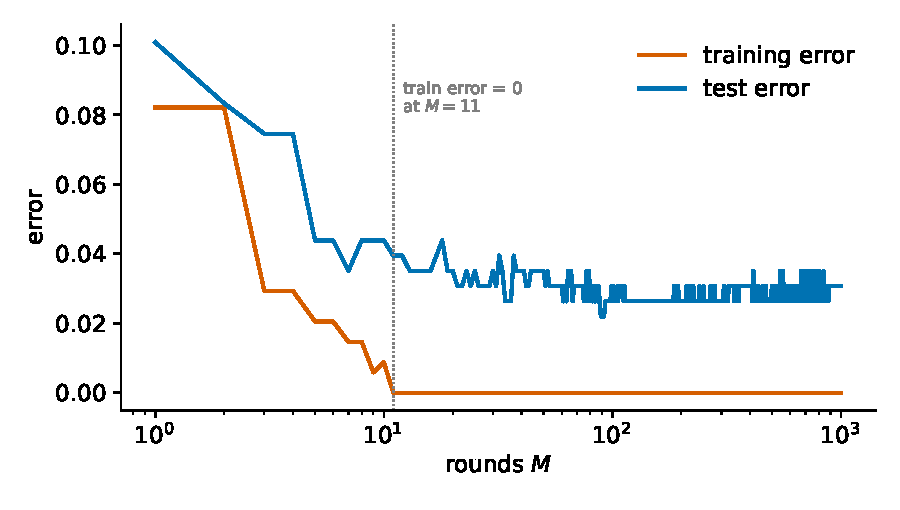
\includegraphics[height=0.55\textheight]{fig_boosting_curves.pdf}
\end{center}
\vspace{-4pt}
AdaBoost with stumps on a benchmark. Training error reaches $0$ early. \textbf{Test error keeps falling
for hundreds of rounds after that.} Adding capacity to a model with zero training error should overfit.
It does not, or not for a long time. Why?
\end{frame}

\begin{frame}{Margins}
Normalize the vote: for $y\in\{\pm1\}$ define the \textbf{margin} of example $i$ as
\[
\mu_i=\frac{y_i\sum_m\alpha_mh_m(\vx_i)}{\sum_m\alpha_m}\ \in[-1,1].
\]
$\mu_i>0$ iff correctly classified; $\mu_i$ near $1$ means a large \emph{weighted majority} of base learners agree.
\begin{claim}{Schapire, Freund, Bartlett \& Lee (1998)}
With probability at least $1-\delta$ over the training sample, for every $\theta>0$,
\[
\Prob_{\text{test}}\bigl[\mu\le0\bigr]\ \le\ \underbrace{\frac1N\sum_i\ind{\mu_i\le\theta}}_{\text{fraction with margin}\le\theta}
+\ O\!\left(\sqrt{\frac{d\,\log^2(N/d)}{N\theta^2}+\frac{\log(1/\delta)}{N}}\right),
\]
where $d$ is the VC dimension of $\Hset_0$. \textbf{The bound does not depend on $M$.}
\end{claim}
\end{frame}

\begin{frame}{Boosting Pushes Margins Up}
\begin{center}
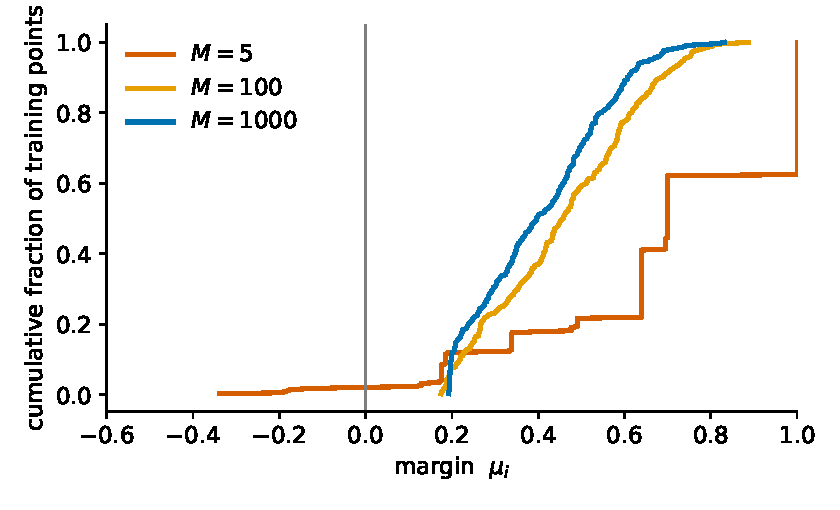
\includegraphics[height=0.5\textheight]{fig_margins.pdf}
\end{center}
\vspace{-4pt}
Cumulative distribution of training margins after 5, 100 and 1000 rounds. Training error is zero from
round $\approx20$ on; what keeps changing is the \emph{distribution}: the mass at small margins moves right.
The bound on the previous slide falls with it, at fixed $M$-independent cost.
\end{frame}

\begin{frame}{Why Margins Grow: The Exponential Loss}
AdaBoost minimizes $\frac1N\sum_ie^{-y_if(\vx_i)}$. Once all $y_if(\vx_i)>0$, this loss is still positive
and still decreasing in each $y_if(\vx_i)$. The algorithm keeps going, and every round puts weight on the
examples with the \emph{smallest} $y_if(\vx_i)$ --- exactly the ones with the smallest margin.
\begin{itemize}
  \item Hinge loss would stop at margin $1$; exponential loss never stops. That is why boosting keeps
        improving test error after training error is zero, and also why it eventually overfits on noisy data
        (it will chase mislabelled points forever).
  \item Log loss (LogitBoost, gradient boosting with binomial deviance) is less aggressive on outliers and
        is the modern default.
  \item The parallel with SVMs is exact: both maximize a margin. The SVM maximizes the $\ell_2$ margin of one
        linear classifier; boosting approximately maximizes the $\ell_1$ margin of a vote.
\end{itemize}
\end{frame}

% =============================================================================
\sectionframe{Summary}
% =============================================================================

\begin{frame}{What We Proved Today}
\begin{enumerate}
  \item Forward stagewise fitting with squared loss fits each base learner to the current residuals.
  \item Gradient boosting is steepest descent in function space, projected onto the base class:
        fit $h_m$ to the pseudo-residuals $-\partial L/\partial f$, then line-search the step.
  \item XGBoost's leaf values $w_j^\star=-G_j/(K_j+\lambda)$ and its split gain follow from a second-order expansion.
  \item Forward stagewise fitting with exponential loss is AdaBoost: the weights are $e^{-y_if_{m-1}(\vx_i)}$,
        the base learner minimizes weighted error, and $\alpha_m=\tfrac12\ln\frac{1-\varepsilon_m}{\varepsilon_m}$.
  \item Training error $\le\prod_m2\sqrt{\varepsilon_m(1-\varepsilon_m)}\le e^{-2\gamma^2M}$.
  \item Test error is governed by the margin distribution, not by $M$; exponential loss keeps increasing margins.
\end{enumerate}
\end{frame}

\begin{frame}{Next}
\textbf{Lab 3 (Wednesday, Rodrigo)} --- information gain by hand, trees vs.\ forests vs.\ gradient boosting on
one dataset, early stopping on $M$, and the AdaBoost trace of this lecture reproduced in code.
\vspace{8pt}

\textbf{Lecture 6 (Monday)} --- no labels at all: $k$-means as coordinate descent, agglomerative clustering,
and principal components as the eigenvectors of the covariance --- the bridge to Machine Learning II.
\vspace{8pt}

\textbf{Reading} --- \emph{ESL} \S10.1--10.6 (AdaBoost, exponential loss), \S10.9--10.12 (gradient boosting,
shrinkage, interaction depth). Schapire et al.\ (1998) for margins; Chen \& Guestrin (2016) for XGBoost.
\end{frame}

\end{document}
